\documentclass{beamer}

\usepackage{tikz}
\usepackage[labelfont=bf]{caption}
\usepackage{booktabs}
\usepackage{caption}
\usepackage{siunitx}
\usepackage{amsmath}

\title{Determining Acceleration due to Gravity through Sonic Time Measurements of Falling Masses}
\author{Henry Oehlrich\and Grace Jiang\and Ansh Agrawal}

\begin{document}
\maketitle

\begin{frame}
    \frametitle{Abstract}
\end{frame}

\begin{frame}
    \frametitle{Experiment Setup}
    \centering
    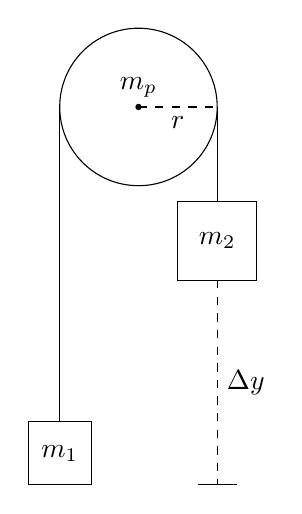
\begin{tikzpicture}
        \draw (0,5) node[above] {$m_p$} circle (1);
        \fill (0,5) circle (0.04);
        \draw[dashed] (0,5) -- (0.5, 5) node[below] {$r$} -- (1,5);

        \draw (1,5) -- (1,3.8);
        \draw (0.5,3.8) rectangle node {$m_2$} ++(1,-1);

        \draw (-1,5) -- (-1,1);
        \draw (-1.4,1) rectangle node {$m_1$} ++(0.8,-0.8);

        \draw[dashed] (1,2.8) -- (1,1.5) node[right] {$\Delta y$} -- (1,0.2);
        \draw (0.75,0.2) -- (1.25,0.2);
    \end{tikzpicture}
    \caption{Lab setup}
    \label{fig:setup}
        &
    \centering
    \begin{tabular}{l|l}
        \toprule
        Symbol & Value \\
        \midrule
        $\Delta y$ & \qty{1.70}{\meter} \\
        $m_1$ & \qty{0.01}{\kilogram} \\
        $g$ & \qty{9.81}{\meter\per\second\squared} \\
        $m_p$ & \qty{0.05}{\kilogram} \\
        $r$ & \qty{0.05}{\meter} \\
        $m_2$ & varied \\
        $t$ & measured \\
    \end{tabular}
    \captionof{table}{Experimental parameters}
    \label{tab:params}
\end{frame}

\begin{frame}
    \frametitle{Materials and Methods}
\end{frame}
\begin{frame}
    \frametitle{Results}
\end{frame}
\begin{frame}
    \frametitle{Discussion}
\end{frame}

\end{document}
